\documentclass{beamer}

\usepackage{amsmath,subcaption}
\usepackage{standalone}


\mode<presentation>
{
  \usetheme{default2}
}

\def\longlongrightarrow{\relbar\joinrel\relbar\joinrel\relbar\joinrel\relbar\joinrel\rightarrow
}
\def\longlonglongrightarrow{\relbar\joinrel\relbar\joinrel\relbar\joinrel\relbar\joinrel\relbar\joinrel\relbar\joinrel\rightarrow
}

\beamertemplatenavigationsymbolsempty

\DeclareMathOperator*{\E}{\mathbb{E}}
\let\Pr\relax
\DeclareMathOperator*{\Pr}{\mathbb{P}}

\newcommand*{\threeemdash}{\rule[0.5ex]{3em}{0.55pt}}

\newcommand{\vertiii}[1]{{\left\vert\kern-0.25ex\left\vert\kern-0.25ex\left\vert #1 \right\vert\kern-0.25ex\right\vert\kern-0.25ex\right\vert}}

\newenvironment{tight-itemize}
{\begin{list}{$\bullet$}
{\itemsep=1pt plus 1pt minus 1pt\parsep=0pt\labelsep=4pt
\parsep=0pt\def\makelabel##1{\hss\llap##1}}}
{\end{list}}

\newcommand{\T}{\mathsf{T}}
\newcommand{\xtail}{x_{\mathrm{tail}}}
\newcommand{\xhead}{x_{\mathrm{head}}}
\newcommand{\filter}{{\sf Filter}\xspace}
\newcommand{\filt}{\textrm{{\sf F}}\xspace}
\newcommand{\hh}{\textrm{{\sf HH}}\xspace}
\newcommand{\GMest}{\mathrm{Est_{GM}}\xspace}
\newcommand{\Est}{\mathrm{Est}\xspace}
\newcommand{\nnz}{\operatornamewithlimits{nnz}}
\newcommand{\red}[1]{\textcolor{red}{#1}}

\newcommand{\black}[1]{\textcolor{black}{#1}}
\definecolor{MyTeal}{rgb}{0,1.0,1.0}
\definecolor{MyPurple}{rgb}{0.635,0.157,1.0} 
\renewcommand{\alert}[1]{\textcolor{MyTeal}{#1}}

\newcommand{\enc}{\mathrm{enc}}
\newcommand{\proj}[1]{tail(#1)}
\newcommand{\inprod}[1]{\left\langle #1 \right\rangle}
\newcommand{\R}{\mathbb{R}}
\newcommand{\sign}{\mathbf{sign}}
\newcommand{\C}{\mathbb{C}}
\newcommand{\indicate}{\mathbf{1}}
\newcommand{\U}{\mathbf{U}}
\newcommand{\Var}{\mathbf{Var}}
\newcommand{\eps}{\varepsilon}
\newcommand{\poly}{\mathrm{poly}}
\newcommand{\polylog}{\mathrm{polylg}}
%\renewcommand{\log}{\lg}
\newcommand{\eqdef}{\mathbin{\stackrel{\rm def}{=}}}
\newcommand{\questionapprox}{\mathbin{\stackrel{\rm ?}{\approx}}}
\newcommand{\important}[1]{\textbf{#1}}
\newcommand{\tO}{\tilde{O}}
\newcommand{\lsb}{\mathrm{lsb}}
\newcommand{\RE}{\mathrm{RE}}
\newcommand{\RoughEst}{\textsc{RoughEstimator}\xspace}
\newcommand{\RoughLEst}{\textsc{RoughL0Estimator}\xspace}
\newcommand{\bzero}{0}
\newcommand{\query}{\texttt{query}}

\newcommand{\centered}[1]{\begin{tabular}{l} #1 \end{tabular}}


\usepackage[english]{babel}
\usepackage{color}
\usepackage{courier}
\usepackage{nicefrac}
\usepackage{xspace}
\usepackage[normalem]{ulem}
\usepackage{pgf}
\usepackage{tikz}
\usepackage{tikz-3dplot}
\usepackage{xifthen}
\usetikzlibrary{positioning,calc} 
\usepackage{colortbl}
\usepackage{bm}
\usepackage[latin1]{inputenc}
\def\floor#1{\lfloor #1 \rfloor}
\def\ceil#1{\lceil #1 \rceil}

\newcommand{\soutthick}[1]{%
    \renewcommand{\ULthickness}{1.2pt}%
       \sout{#1}%
    \renewcommand{\ULthickness}{.4pt}% Resetting to ulem default
}

\DeclareMathOperator*{\argmin}{\mathrm{argmin}}

\newtheorem{conjecture}[theorem]{Conjecture}

\title[Logarithms\hspace{2em}\insertframenumber/
\inserttotalframenumber]{Logarithms}

 \author{Jelani Nelson\\UC Berkeley}
                                % only with lots of authors)

\date[\today]
{July 17, 2023}

\tdplotsetmaincoords{70}{120} % set viewpoint 
\tdplotsetrotatedcoords{0}{0}{0} %<- rotate around (z,y,z)
\begin{document}

\begin{frame}
  \titlepage

  \begin{center}
    {\tiny \alert{JamCoders 2023}}
  \end{center}
\end{frame}

\begin{frame}
  ``Logarithm'' is the opposite of ``exponential''

  \pause

  \bigskip

  \begin{itemize}
  \item $10^3 = 1000$
  \item[] $\log_{10}(1000) = 3$
    \item[] \alert{``the logarithm base $10$ of $1000$ is $3$''}
    \item[]
  \item $2^5 = 32$
  \item[] $\log_2(32) = 5$
        \item[] \alert{``the logarithm base $2$ of $32$ is $5$''}
    \end{itemize}
  \end{frame}

  \begin{frame}
    \begin{columns}
      \column{2in}
    \begin{itemize}
    \item[] $\log_{10}(1) = 1$
    \item[] $\log_{10}(10) = 2$
    \item[] $\log_{10}(100) = 3$
    \item[] $\log_{10}(1{,}000) = 4$
    \item[] $\log_{10}(10{,}000) = 5$
    \item[] $\log_{10}(100{,}000) = 6$
    \item[] $\log_{10}(1{,}000{,}000) = 7$
    \item[] $\log_{10}(10{,}000{,}000) = 8$
    \item[] $\log_{10}(100{,}000{,}000) = 9$
    \item[] $\log_{10}(1{,}000{,}000{,}000) = 10$      
    \end{itemize}
    \column{3in}
    \textcolor{yellow}{When the \alert{base} is 10, and the argument $x$ is a power of $10$, $\log_{10}(x)$ counts number of zeroes.}
    \end{columns}
  \end{frame}

  \begin{frame}
    \begin{center}
      \scalebox{0.17}{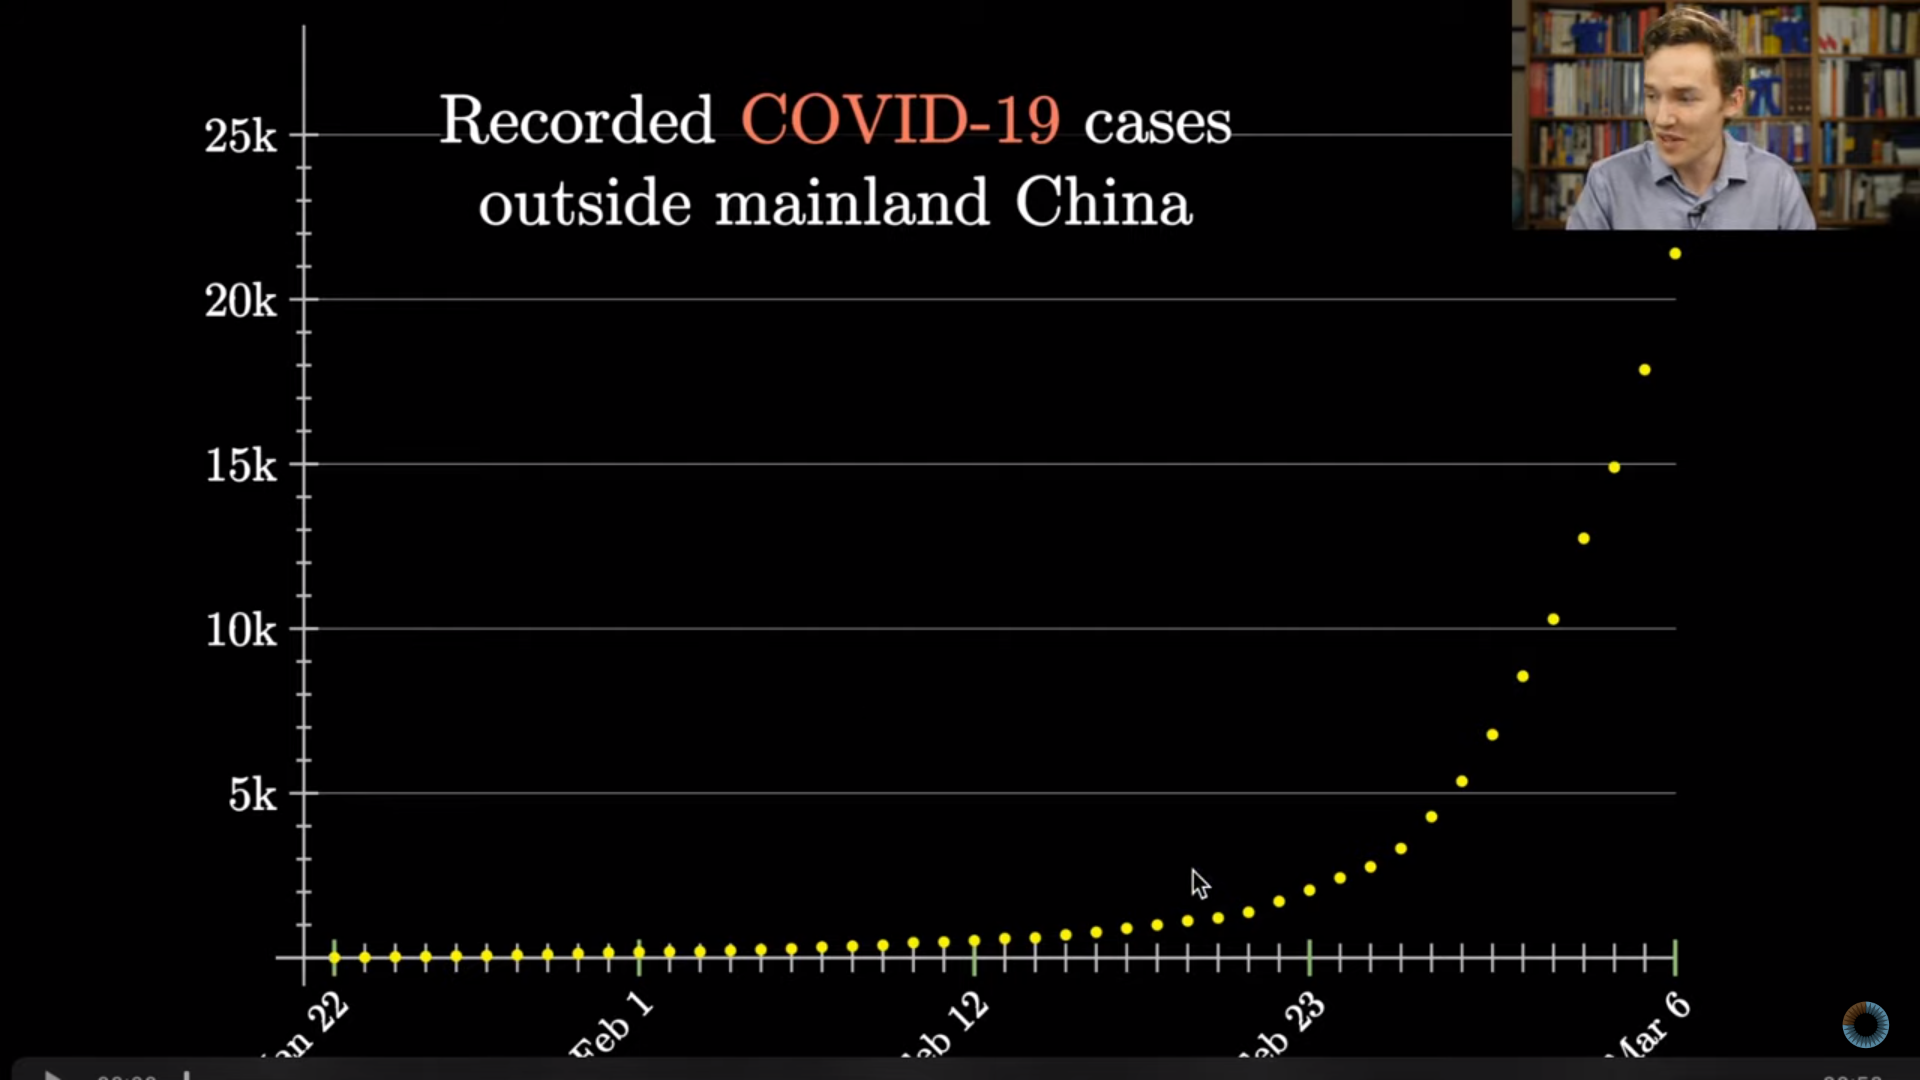
\includegraphics{exponential}}\\
      $f(x) = $ number of recorded COVID-19 cases on day $x$\\
      \alert{source:} 3Blue1Brown {\tiny (\url{https://www.youtube.com/watch?v=cEvgcoyZvB4})}
      \end{center}
    \end{frame}
    
    \begin{frame}
    \begin{center}
      \scalebox{0.17}{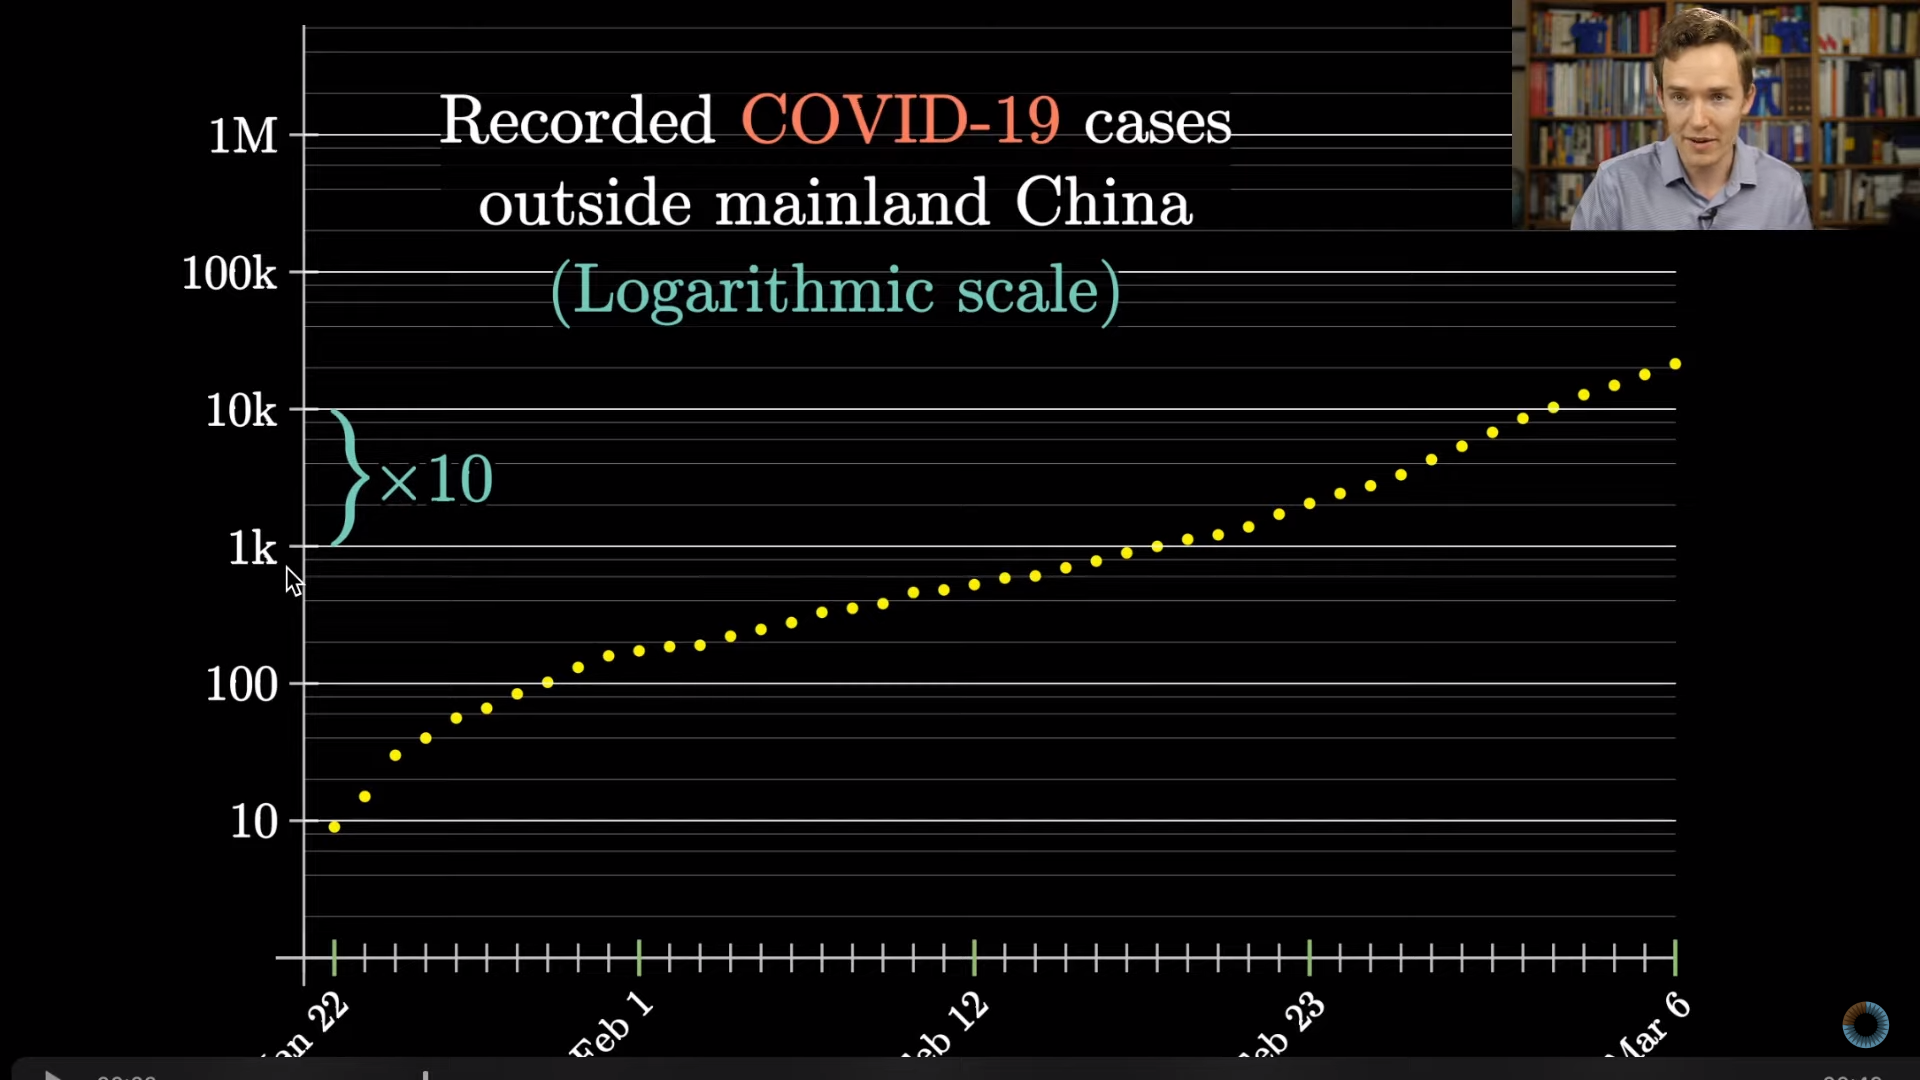
\includegraphics{log_scale}}\\
      $g(x) = \log_{10}(\text{number of recorded COVID-19 cases on day }x)$\\
      \alert{source:} 3Blue1Brown {\tiny (\url{https://www.youtube.com/watch?v=cEvgcoyZvB4})}
      \end{center}
    \end{frame}

    \begin{frame}
    \begin{center}
      \scalebox{0.17}{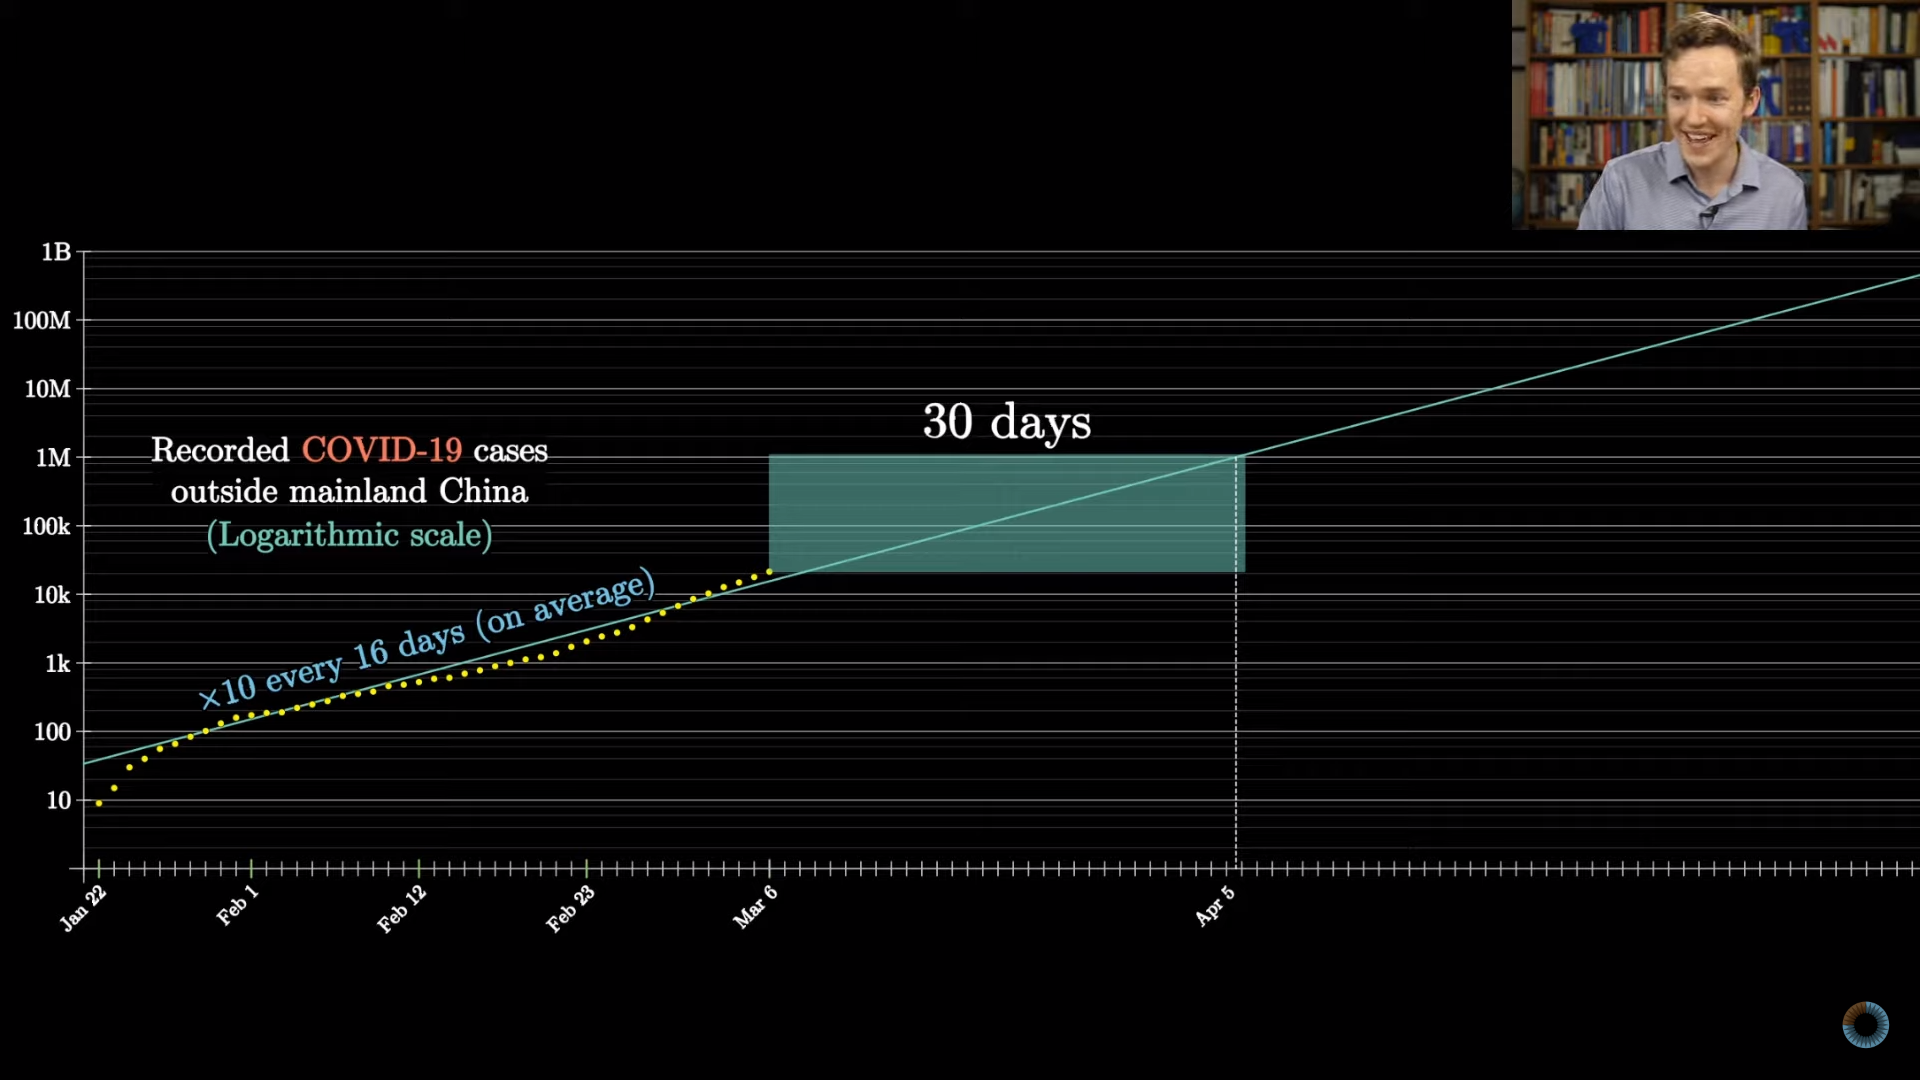
\includegraphics{prediction}}\\
      On what day do we expect to cross 1 million recorded cases?\\
      \alert{source:} 3Blue1Brown {\tiny (\url{https://www.youtube.com/watch?v=cEvgcoyZvB4})}
      \end{center}
    \end{frame}

    \begin{frame}
      $\times 10$ every 16 days $\Longrightarrow$ what is the daily rate of increase? $\ldots$

      \pause
      
      \bigskip     
      
      \begin{itemize}
      \item $r^{16} = 10$
        \item[] $\Longrightarrow r = 10^{1/16} = 1.15478198469\ldots$
        \end{itemize}

        \pause

        \bigskip

        Starting from day $1$, how long before 1 million cases?\\

        \begin{center}
        $1.1548^x = 1{,}000{,}000$ means $x = \log_{1.1548}(1{,}000{,}000)$ days\\
        \alert{(96 days)}
        \end{center}
      \end{frame}

      \begin{frame}
        \frametitle{Product rule for logarithms}
        \begin{center}
          $\log_a(b\cdot c) = ?$
        \end{center}

        \pause

        Go back to examples:
        \begin{align*}
          \log_{10}(\underbrace{100}_2\cdot \underbrace{1000}_3) &= \log_{10}(100{,}000)\\
                                     &= 5\\
        \end{align*}

        \pause
        \vspace{-.3in}\alert{Guess:} $\log_a(b\cdot c) = \log_a(b) + \log_a(c)$

        \pause

        \bigskip

        Indeed, $a^x = b, a^y = c$ means $a^{x+y} = b\cdot c$\\
        ($x$ is $\log_a(b)$ and $y$ is $\log_a(c)$)
      \end{frame}

            \begin{frame}
              \frametitle{Exponent rule for logarithms}
                      \begin{center}
          $\log_a(b^n) = ?$
        \end{center}

        \pause

        Go back to examples:
        \begin{align*}
          \log_{10}(100^3) &= \log_{10}(\underbrace{100}_2\cdot \underbrace{100}_2 \cdot \underbrace{100}_2)\\
                                          &= \log_{10}(1{,}000{,}000)\\
          &= 6\ (\text{which is } 3\times 2)
        \end{align*}

        \pause
        \vspace{-.1in}\alert{Guess:} $\log_a(b^n) = n\cdot \log_a(b)$

        \pause

        \bigskip

        Indeed, if $a^x = b$ then $b^n = (a^x)^n = a^{n\cdot x}$\\
        ($x$ is $\log_a(b)$)
        
      \end{frame}

      \begin{frame}
        \frametitle{Change of base for logarithms}

        \begin{center}
          What is $\log_b(a)$ in terms of $\log_a(b)$?
        \end{center}

        \pause

        Go back to examples:
        $$
        \log_{1000}(10) = 1/3
        $$
        since $\sqrt[3]{1000} = 10$

        \pause
        \bigskip
       \alert{Guess:} $\log_b(a) = 1 / \log_a(b)$

        \pause

        \bigskip

        Indeed, $a^x = b$ means $b^{1/x} = a$
      \end{frame}


\end{document}
